\documentclass[a4paper,12pt]{article} % This defines the style of your paper

\usepackage[top = 2.5cm, bottom = 2.5cm, left = 2.5cm, right = 2.5cm]{geometry} 

% Unfortunately, LaTeX has a hard time interpreting German Umlaute. The following two lines and packages should help. If it doesn't work for you please let me know.
\usepackage[T1]{fontenc}
\usepackage[utf8]{inputenc}
\usepackage{pifont}
% \usepackage{ctex}
\usepackage{amsthm, amsmath, amssymb, mathrsfs,mathtools}

% Defining a new theorem style without italics
\newtheoremstyle{nonitalic}% name
  {\topsep}% Space above
  {\topsep}% Space below
  {\upshape}% Body font
  {}% Indent amount
  {\bfseries}% Theorem head font
  {.}% Punctuation after theorem head
  {.5em}% Space after theorem head
  {}% Theorem head spec (can be left empty, meaning ‘normal`)
  
\theoremstyle{nonitalic}
% Define new 'solution' environment
\newtheorem{innercustomsol}{Solution}
\newenvironment{solution}[1]
  {\renewcommand\theinnercustomsol{#1}\innercustomsol}
  {\endinnercustomsol}

% Custom counter for the solutions
\newcounter{solutionctr}
\renewcommand{\thesolutionctr}{(\alph{solutionctr})}

% Environment for auto-numbering with custom format
\newenvironment{autosolution}
  {\stepcounter{solutionctr}\begin{solution}{\thesolutionctr}}
  {\end{solution}}


\newtheorem{problem}{Problem}
\usepackage{color}

% The following two packages - multirow and booktabs - are needed to create nice looking tables.
\usepackage{multirow} % Multirow is for tables with multiple rows within one cell.
\usepackage{booktabs} % For even nicer tables.

% As we usually want to include some plots (.pdf files) we need a package for that.
\usepackage{graphicx} 
\usepackage{subfigure}


% The default setting of LaTeX is to indent new paragraphs. This is useful for articles. But not really nice for homework problem sets. The following command sets the indent to 0.
\usepackage{setspace}
\setlength{\parindent}{0in}
\usepackage{longtable}

% Package to place figures where you want them.
\usepackage{float}

% The fancyhdr package let's us create nice headers.
\usepackage{fancyhdr}

\usepackage{fancyvrb}

%Code environment 
\usepackage{listings} % Required for insertion of code
\usepackage{xcolor} % Required for custom colors

% Define colors for code listing
\definecolor{codegreen}{rgb}{0,0.6,0}
\definecolor{codegray}{rgb}{0.5,0.5,0.5}
\definecolor{codepurple}{rgb}{0.58,0,0.82}
\definecolor{backcolour}{rgb}{0.95,0.95,0.92}

% Code listing style named "mystyle"
\lstdefinestyle{mystyle}{
    backgroundcolor=\color{backcolour},   
    commentstyle=\color{codegreen},
    keywordstyle=\color{magenta},
    numberstyle=\tiny\color{codegray},
    stringstyle=\color{codepurple},
    basicstyle=\ttfamily\footnotesize, % Change to serif font
    columns=fullflexible, % make sure to use fixed-width font, CM typewriter is NOT fixed width
    numbers=left,
    stepnumber=1,
    numbersep=10pt,
    numberfirstline=true,
    numberblanklines=true,
    tabsize=4,
    lineskip=-1.5pt,
    extendedchars=true,
    breaklines=true,
    identifierstyle=, % using emph or index keywords
    showstringspaces=false,
    showtabs=false,
    upquote=false,
    texcl=true % interpet comments as LaTeX
}

\lstset{style=mystyle}


%%%%%%%%%%%%%%%%%%%%%%%%%%%%%%%%%%%%%%%%%%%%%%%%
% 3. Header (and Footer)
%%%%%%%%%%%%%%%%%%%%%%%%%%%%%%%%%%%%%%%%%%%%%%%%

% To make our document nice we want a header and number the pages in the footer.

\pagestyle{fancy} % With this command we can customize the header style.

\fancyhf{} % This makes sure we do not have other information in our header or footer.

\lhead{\footnotesize EI035 Econometrics II}% \lhead puts text in the top left corner. \footnotesize sets our font to a smaller size.

%\rhead works just like \lhead (you can also use \chead)
\rhead{\footnotesize Jingle Fu} %<---- Fill in your lastnames.

% Similar commands work for the footer (\lfoot, \cfoot and \rfoot).
% We want to put our page number in the center.
\cfoot{\footnotesize \thepage}
\IfFileExists{upquote.sty}{\usepackage{upquote}}{}
\begin{document}


\thispagestyle{empty} % This command disables the header on the first page. 

\begin{tabular}{p{15.5cm}} % This is a simple tabular environment to align your text nicely 
  {\large \bf EI035 Econometrics II}                 \\
  The Graduate Institute, Spring 2025, Marko Mlikota \\
  \hline % \hline produces horizontal lines.
  \\
\end{tabular} % Our tabular environment ends here.

\vspace*{0.3cm} % Now we want to add some vertical space in between the line and our title.

\begin{center} % Everything within the center environment is centered.
  {\Large \bf PS2 Solutions} % <---- Don't forget to put in the right number
  \vspace{2mm}

  % YOUR NAMES GO HERE
  {\bf Jingle Fu} % <---- Fill in your names here!

\end{center}

\vspace{0.4cm}
\setstretch{1.2}


\section*{Problem 1: Dynamic Panel Data with Correlated Random Effects}

\subsection*{Model}
\begin{equation*}
  y_{it} = \alpha_i + \rho y_{it-1} + u_{it}, \quad u_{it} \sim iid \mathcal{N}(0, 1)
\end{equation*}

\subsection*{CRE Distribution}
\begin{equation*}
  \alpha_i | (y_{i0}, \phi) \sim \mathcal{N}(\phi y_{i0}, 1)
\end{equation*}

\subsection*{(a) The Incidental Parameter Problem (IPP)}
The incidental parameter problem arises in panel data models when the number of parameters to be estimated grows with the sample size $N$.
Here, the unit-specific effects $\alpha_1, ..., \alpha_N$ are the incidental parameters.

In a dynamic panel (where $y_{it-1}$ is a regressor),
the standard Fixed Effects (Within) estimator or the naive MLE for $\alpha_i$ and $\rho$ yields inconsistent estimates for $\rho$ when $N \to \infty$ but $T$ remains fixed.

Treating $\{\alpha_i\}_{i=1}^n$ as fixed parameters in FE--ML yields
\[
  \ell_i(\alpha_i,\rho)
  \;=\;
  -\frac{T}{2}\log(2\pi)
  -\frac{1}{2}\sum_{t=1}^T\big(y_{it}-\alpha_i-\rho\,y_{i,t-1}\big)^2,
\]
and the first-order condition for $\alpha_i$ is
\[
  \frac{\partial \ell_i}{\partial \alpha_i}
  \;=\;
  \sum_{t=1}^T\big(y_{it}-\alpha_i-\rho\,y_{i,t-1}\big)
  \;=\;0
  \;=\;
  T\,\hat{\alpha}_i - \sum_{t=1}^T\big(y_{it}-\rho\,y_{i,t-1}\big),
\]
hence
\[
  \hat{\alpha}_i
  \;=\;
  \frac{1}{T}\sum_{t=1}^T\big(y_{it}-\rho\,y_{i,t-1}\big)
  \;=\;
  \alpha_i
  \;+\; \frac{1}{T}\sum_{t=1}^T u_{it}.
\]
Because $y_{i,t-1}$ embeds $\alpha_i$, the estimation error $\hat\alpha_i-\alpha_i$ remains correlated with $y_{i,t-1}$ when $T$ is fixed:
\[
  \mathrm{Cov}\!\big(y_{i,t-1},\,\hat{\alpha}_i-\alpha_i\big)
  \;\neq\; 0 \quad\text{for fixed $T$}.
\]
Thus, as $n\to\infty$ with $T$ fixed, the FE estimator $\hat\rho$ has an $O(1/T)$ bias.
In contrast, the CRE--Bayesian route treats $\alpha_i$ hierarchically so that inference on $(\phi,\rho)$ does not suffer from the IPP.

% This happens because the estimation error of $\alpha_i$ (which does not vanish as $N \to \infty$) is correlated with the regressor $y_{it-1}$ (since $y_{it-1}$ contains $\alpha_i$).
% This induces a downward bias in the estimate of $\rho$, commonly known as the \textbf{Nickell Bias} (of order $1/T$).

\subsection*{(b) Integrating out $\alpha_i$}

% \paragraph{Step 1: Cumulative multiplication of conditional densities}
Given $\tilde y_{it}=\alpha_i+u_{it}$ and $u_{it}\sim\mathcal{N} (0,1)$, we have:
\[
  p(\tilde y_{it}\mid \alpha_i)=\frac{1}{\sqrt{2\pi}}\exp\Big(-\tfrac12(\tilde y_{it}-\alpha_i)^2\Big).
\]
Due to independence across $t$ (conditional on $\alpha_i$):
\begin{align*}
  p(\tilde{\mathbf y}_i\mid \alpha_i) & = \prod_{t=1}^T \frac{1}{\sqrt{2\pi}}\exp\Big(-\tfrac12(\tilde y_{it}-\alpha_i)^2\Big) \\
                                      & = (2\pi)^{-T/2}\exp\Big(-\tfrac12\sum_{t=1}^T(\tilde y_{it}-\alpha_i)^2\Big).
\end{align*}

% \paragraph{Step 2: Multiplication with the prior to obtain the joint kernel}
The prior (CRE) is:
\[
  p(\alpha_i\mid y_{i0},\phi)=\frac{1}{\sqrt{2\pi}}\exp\Big(-\tfrac12(\alpha_i-\phi y_{i0})^2\Big).
\]
Thus:
\[
  \begin{aligned}
    p(\tilde{\mathbf y}_i,\alpha_i\mid y_{i0},\phi,\rho)
     & =p(\tilde{\mathbf y}_i\mid \alpha_i)\,p(\alpha_i\mid y_{i0},\phi)                                                                                           \\
     & =(2\pi)^{-(T+1)/2}\exp\Big(-\tfrac12\,\underbrace{\Big[\sum_{t=1}^T(\tilde y_{it}-\alpha_i)^2+(\alpha_i-\phi y_{i0})^2\Big]}_{\mathcal{Q} (\alpha_i)}\Big).
  \end{aligned}
\]

% \paragraph{Step 3: Expanding $\mathcal{Q} (\alpha_i)$ to ``complete the square''}
\[
  \sum_{t=1}^T(\tilde y_{it}-\alpha_i)^2
  =\sum_{t=1}^T\tilde y_{it}^2-2\alpha_i\sum_{t=1}^T\tilde y_{it}+T\alpha_i^2,
\]
\[
  (\alpha_i-\phi y_{i0})^2=\alpha_i^2-2\phi y_{i0}\alpha_i+\phi^2y_{i0}^2.
\]
Summing these yields:
\[
  \mathcal{Q} (\alpha_i)
  =(T+1)\alpha_i^2-2\alpha_i\Big(\sum_{t=1}^T\tilde y_{it}+\phi y_{i0}\Big)
  +\Big(\sum_{t=1}^T\tilde y_{it}^2+\phi^2y_{i0}^2\Big).
\]
Let:
\[
  c\equiv T+1,\quad b\equiv \sum_{t=1}^T\tilde y_{it}+\phi y_{i0},\quad a\equiv \sum_{t=1}^T\tilde y_{it}^2+\phi^2y_{i0}^2,
\]
then:
\[
  \mathcal{Q} (\alpha_i)=c\alpha_i^2-2b\alpha_i+a
  =c\Big(\alpha_i-\frac{b}{c}\Big)^2+\Big(a-\frac{b^2}{c}\Big).
\]

% \paragraph{Step 4: One-dimensional Gaussian integration with respect to $\alpha_i$}
\[
  \begin{aligned}
    p(\tilde{\mathbf y}_i\mid y_{i0},\phi,\rho)
     & =\int_{-\infty}^{\infty} p(\tilde{\mathbf y}_i,\alpha_i\mid\cdot)\,d\alpha_i                                                                                    \\
     & =(2\pi)^{-(T+1)/2}\exp\Big(-\tfrac12\Big(a-\tfrac{b^2}{c}\Big)\Big)\int_{-\infty}^{\infty}\exp\Big(-\tfrac12 c\big(\alpha_i-\tfrac{b}{c}\big)^2\Big)\,d\alpha_i \\
     & =(2\pi)^{-(T+1)/2}\exp\Big(-\tfrac12\Big(a-\tfrac{b^2}{c}\Big)\Big)\cdot\sqrt{\frac{2\pi}{c}}                                                                   \\
     & =(2\pi)^{-T/2}\,c^{-1/2}\,\exp\Big(-\tfrac12\Big[a-\tfrac{b^2}{c}\Big]\Big).
  \end{aligned}
\]
Substituting $c=T+1$ back:
\[
  p(\tilde{\mathbf y}_i\mid y_{i0},\phi,\rho)
  =(2\pi)^{-T/2}(T+1)^{-1/2} \exp\Big(-\tfrac12 \Big[\sum_{t=1}^T \tilde y_{it}^2 + \phi^2y_{i0}^2 - \frac{\big(\sum_{t=1}^T \tilde y_{it} + \phi y_{i0} \big)^2}{T+1}\Big]\Big).
\]

% \paragraph{Step 5: Rearranging the exponent into Multivariate Normal Mahalanobis form}
Note that:
\[
  \sum_{t=1}^T \tilde y_{it}^2 = \tilde{\mathbf y}_i^\top\tilde{\mathbf y}_i,\qquad
  \sum_{t=1}^T \tilde y_{it} = \mathbf 1^\top \tilde{\mathbf y}_i.
\]
Let $\boldsymbol \mu\equiv \phi y_{i0}\mathbf 1$ and
\[
  \boldsymbol \Omega \equiv I_T + \mathbf 1 \mathbf 1^\top \Rightarrow\, \boldsymbol \Omega^{-1} = I_T - \frac{1}{T+1} \mathbf 1 \mathbf 1^\top, \quad
  |\boldsymbol \Omega| = (1+T)\cdot 1^{T-1} = T + 1.
\]

\begin{align*}
  \mathcal{Q} & = \sum_{t=1}^T \tilde y_{it}^2 + \phi^2y_{i0}^2 - \frac{\big(\sum_{t=1}^T \tilde y_{it} + \phi y_{i0} \big)^2}{T+1}                            \\
              & = \tilde{\mathbf y}_i^\top \tilde{\mathbf y}_i
  - \frac{(\sum \tilde y_{it})^2}{T+1}
  - \frac{2 \phi y_{i0}}{T+1}\sum \tilde y_{it}
  + \phi^2 y_{i0}^2 \Big(1-\frac{1}{T+1}\Big)                                                                                                                  \\
              & = \tilde{\mathbf y}_i^\top \tilde{\mathbf y}_i
  - \frac{( \sum \tilde y_{it})^2}{T+1}
  + \Big[(\phi y_{i0})^2T - \frac{(\phi y_{i0})^2T^2}{T+1}\Big]
  + \Big[-2 \phi y_{i0} \sum \tilde y_{it} + \frac{2\phi y_{i0}T}{T+1} \sum \tilde y_{it} \Big]                                                                \\
              & = \tilde{\mathbf y}_i^\top \tilde{\mathbf y}_i
  + (\phi y_{i0})^2 T
  - 2 \phi y_{i0} \sum \tilde y_{it}
  - \frac{1}{T+1} \Big[ ( \sum \tilde y_{it})^2 - 2 \phi y_{i0}T \sum \tilde y_{it} + (\phi y_{i0})^2T^2\Big]                                                  \\
              & = \tilde{\mathbf y}_i^\top \tilde{\mathbf y}_i-2(\phi y_{i0}) \mathbf 1^\top \tilde{\mathbf y}_i+(\phi y_{i0})^2 \mathbf 1^\top \mathbf 1
  - \frac{1}{T+1} \big( \mathbf 1^\top \tilde{\mathbf y}_i-\phi y_{i0} \mathbf 1^\top \mathbf 1 \big)^2                                                        \\
              & = \tilde{\mathbf y}_i^\top \tilde{\mathbf y}_i-2 \boldsymbol \mu^\top \tilde{\mathbf y}_i + \boldsymbol \mu^\top \boldsymbol \mu
  - \frac{1}{T+1} \big(\mathbf 1^\top \tilde{\mathbf y}_i - \mathbf 1^\top \boldsymbol \mu \big)^2                                                             \\
              & = (\tilde{\mathbf y}_i - \boldsymbol \mu)^\top (\tilde{\mathbf y}_i - \boldsymbol \mu)
  - \frac{1}{T+1} \big[\mathbf 1^\top (\tilde{\mathbf y}_i - \boldsymbol \mu)\big]^2                                                                           \\
              & = (\tilde{\mathbf y}_i - \boldsymbol \mu)^\top \Big(I_T - \tfrac{1}{T+1} \mathbf 1 \mathbf 1^\top \Big)(\tilde{\mathbf y}_i - \boldsymbol \mu) \\
              & = (\tilde{\mathbf y}_i - \boldsymbol \mu)^\top \boldsymbol \Omega^{-1} (\tilde{\mathbf y}_i - \boldsymbol \mu)
\end{align*}

Therefore:
\[
  p(\tilde{\mathbf y}_i\mid y_{i0},\phi,\rho)
  = (2\pi)^{-T/2} |\boldsymbol \Omega|^{-1/2}
  \exp \Big( -\tfrac12 (\tilde{\mathbf y}_i - \boldsymbol \mu)^\top \boldsymbol \Omega^{-1} (\tilde{\mathbf y}_i - \boldsymbol \mu) \Big).
\]

\subsection*{(c) Consistency of $(\phi, \rho)$}
The sample log-likelihood is:
\[
  \ell(\phi,\rho)=\sum_{i=1}^n\ell_i(\phi,\rho),
\]
where (derived directly from the above equation):
\[
  \ell_i=-\frac{T}{2}\log(2\pi)-\frac{1}{2}\log(T+1)-\frac{1}{2}\,
  (\tilde{\mathbf y}_i-\phi y_{i0}\mathbf 1)^\top
  \Big(I_T-\frac{1}{T+1}\mathbf 1\mathbf 1^\top\Big)
  (\tilde{\mathbf y}_i-\phi y_{i0}\mathbf 1).
\]

\paragraph{Score w.r.t. $\phi$:}
\[
  \begin{aligned}
    \frac{\partial \ell}{\partial \phi}
     & =\sum_{i=1}^n \frac{\partial \ell_i}{\partial \phi}
    =\sum_{i=1}^n \frac{1}{2}\cdot 2\,y_{i0}\mathbf 1^\top\Big(I-\tfrac{1}{T+1}\mathbf 1\mathbf 1^\top\Big)
    (\tilde{\mathbf y}_i-\phi y_{i0}\mathbf 1)\cdot(+1)                                      \\
     & =\sum_{i=1}^n y_{i0}\,\mathbf 1^\top\Big(I-\tfrac{1}{T+1}\mathbf 1\mathbf 1^\top\Big)
    (\tilde{\mathbf y}_i-\phi y_{i0}\mathbf 1).
  \end{aligned}
\]
Setting this score to 0 implies:
\[
  \sum_i y_{i0}\,\mathbf 1^\top\Big(I-\tfrac{1}{T+1}\mathbf 1\mathbf 1^\top\Big)\tilde{\mathbf y}_i
  =\phi\sum_i y_{i0}^2\,\mathbf 1^\top\Big(I-\tfrac{1}{T+1}\mathbf 1\mathbf 1^\top\Big)\mathbf 1.
\]
In the RHS, $\mathbf 1^\top(I-\frac{1}{T+1}\mathbf 1\mathbf 1^\top)\mathbf 1 = \mathbf 1^\top\mathbf 1-\frac{1}{T+1}\mathbf 1^\top\mathbf 1\,\mathbf 1^\top\mathbf 1 = T-\frac{T^2}{T+1}=\frac{T}{T+1}$.

\paragraph{Score w.r.t. $\rho$:}
\[
  \tilde{\mathbf y}_i=\mathbf y_i-\rho\,\mathbf L_i\mathbf y_i\quad\Rightarrow\quad
  \frac{\partial \tilde{\mathbf y}_i}{\partial \rho}=-(\mathbf L_i\mathbf y_i).
\]
Thus:
\[
  \frac{\partial \ell}{\partial \rho}
  =\sum_i \big[-(\mathbf L_i\mathbf y_i)\big]^\top\Big(I-\tfrac{1}{T+1}\mathbf 1\mathbf 1^\top\Big)
  (\tilde{\mathbf y}_i-\phi y_{i0}\mathbf 1)=0.
\]
These two \textbf{moment equations} have an \textbf{expectation} of 0 at the true values $(\phi_0,\rho_0)$.
As $n\to\infty$, the average log-likelihood converges by the Law of Large Numbers to its expectation,
which is uniquely maximized at the true parameter values $(\phi_0,\rho_0)$.
This avoids the incidental parameter problem because the individual effects $\alpha_i$ have been integrated out.

\subsection*{(d) Estimation of $\alpha_i$}
In a Bayesian (or Correlated Random Effects) framework, since we cannot estimate $\alpha_i$ consistently (it does not converge to a point),
we estimate its conditional posterior distribution or its conditional expectation given the data.

The posterior kernel is:
\begin{align*}
  p(\alpha_i\mid \tilde{\mathbf y}_i,y_{i0},\phi,\rho)
   & \propto p(\tilde{\mathbf y}_i\mid \alpha_i)\,p(\alpha_i\mid y_{i0},\phi)       \\
   & \propto \exp\Big(-\tfrac12\sum_{t=1}^T(\tilde y_{it}-\alpha_i)^2\Big)\cdot
  \exp\Big(-\tfrac12(\alpha_i-\phi y_{i0})^2\Big)                                   \\
   & = \exp\Big(-\tfrac12\big[c(\alpha_i-\tfrac{b}{c})^2+a-\tfrac{b^2}{c}\big]\Big)
  \quad(\text{see definitions of } c,b,a \text{ above}).
\end{align*}

Therefore:
\[
  \alpha_i\mid \tilde{\mathbf y}_i,y_{i0},\phi,\rho\ \sim\
  \mathcal{N} \Big( \frac{\sum_{t=1}^T\tilde y_{it}+\phi y_{i0}}{T+1}, \frac{1}{T+1} \Big)
\]
The posterior mean (Bayes estimator) is:
\begin{align*}
  \hat{\alpha }_i & = \mathbb{E}[\alpha_i\mid \tilde{\mathbf y}_i,y_{i0},\phi,\rho] \\
                  & = \frac{\sum_{t=1}^T\tilde y_{it}+\phi y_{i0}}{T+1}             \\
                  & = \frac{\sum_{t=1}^T(y_{it}-\rho y_{i,t-1})+\phi y_{i0}}{T+1}.
\end{align*}
we would first estimate $(\hat{\phi}, \hat{\rho})$ from the marginal likelihood,
then plug them into the above expression to get $\hat{\alpha}_i$.

\section*{Problem 2: State-Space Model}

\subsection*{Model}
\begin{align*}
  y_t & = \lambda s_t + u_t                                                                             \\
  s_t & = \phi s_{t-1} + \varepsilon_t                                                                  \\
  u_t & \sim \mathcal{N}(0,1), \quad \varepsilon_t \sim \mathcal{N}(0,1), \quad u_t \perp \varepsilon_t
\end{align*}

\subsection*{(a) Autocovariance Function for $y_t$}
Assuming stationarity ($|\phi| < 1$), the state process $s_t$ has the following autocovariance function:
\begin{align*}
  \gamma_s(0) & = \mathrm{Var}(s_t) = \frac{1}{1-\phi^2},                                                    \\
  \gamma_s(h) & = \mathrm{Cov}(s_t, s_{t-h}) = \phi^h \gamma_s(0) = \frac{\phi^h}{1-\phi^2}, \quad h \geq 1.
\end{align*}

For the observed process $y_t = \lambda s_t + u_t$, with $u_t \sim \mathrm{iid}N(0,1)$ independent of $\{\varepsilon_t\}$ (and hence of $\{s_t\}$), the autocovariance function is:
\begin{align*}
  \gamma_y(0) & = \mathrm{Var}(y_t) = \mathrm{Var}(\lambda s_t + u_t) = \lambda^2\mathrm{Var}(s_t) + \mathrm{Var}(u_t)                                                                                                                  \\
              & = \lambda^2 \frac{1}{1-\phi^2} + 1 = \frac{\lambda^2}{1-\phi^2} + 1,                                                                                                                                                    \\[6pt]
  \gamma_y(h) & = \mathrm{Cov}(y_t, y_{t-h}) = \mathrm{Cov}(\lambda s_t + u_t, \lambda s_{t-h} + u_{t-h})                                                                                                                               \\
              & = \lambda^2 \mathrm{Cov}(s_t, s_{t-h}) + \underbrace{\lambda\mathrm{Cov}(s_t, u_{t-h})}_{=0} + \underbrace{\lambda\mathrm{Cov}(u_t, s_{t-h})}_{=0} + \underbrace{\mathrm{Cov}(u_t, u_{t-h})}_{=0 \text{ for } h \neq 0} \\
              & = \lambda^2 \gamma_s(h) = \frac{\lambda^2 \phi^h}{1-\phi^2}, \quad h \geq 1.
\end{align*}

Thus, the autocovariance function of $y_t$ is:
\[
  \gamma_y(h) =
  \begin{cases}
    \dfrac{\lambda^2}{1-\phi^2} + 1,    & h = 0,    \\[10pt]
    \dfrac{\lambda^2 \phi^h}{1-\phi^2}, & h \geq 1.
  \end{cases}
\]
% Assuming stationarity ($|\phi| < 1$), the variance of the state $s_t$ is $\text{Var}(s_t) = \frac{1}{1-\phi^2}$.
% The covariance of the state is $\gamma_k^s = E[s_t s_{t-k}] = \phi^k \frac{1}{1-\phi^2}$.

% For $y_t$:

% \textbf{Variance ($\gamma_0$):}
% \begin{equation*}
%   \gamma_0 = E[(\lambda s_t + u_t)^2] = \lambda^2 \text{Var}(s_t) + \text{Var}(u_t) = \frac{\lambda^2}{1-\phi^2} + 1
% \end{equation*}

% \textbf{Autocovariance ($\gamma_k, k \ge 1$):}
% \begin{align*}
%   \gamma_k & = E[y_t y_{t-k}] = E[(\lambda s_t + u_t)(\lambda s_{t-k} + u_{t-k})] \\
%            & = \lambda^2 E[s_t s_{t-k}] = \lambda^2 \frac{\phi^k}{1-\phi^2}
% \end{align*}
% Since $u_t$ is independent of $s_{t-k}$, $u_{t-k}$, and $s_t$ (for $k \ge 1$).

% \[
%   s_t=\sum_{j=0}^\infty \phi^j\varepsilon_{t-j}
%   \Rightarrow \mathbb E[s_t]=0,\
%   \mathbb V[s_t]=\sum_{j\ge0}\phi^{2j}=\frac{1}{1-\phi^2},
% \]
% \[
%   \mathrm{Cov}(s_t,s_{t-k})
%   =\sum_{j\ge0}\sum_{\ell\ge0}\phi^{j+\ell}\,\mathrm{Cov}(\varepsilon_{t-j},\varepsilon_{t-k-\ell})
%   =\sum_{j\ge0}\phi^{j+k+j}=\frac{\phi^k}{1-\phi^2}.
% \]
% \[
%   y_t=\lambda s_t+u_t\ \perp\ s_t
%   \Rightarrow
%   \gamma_0=\mathbb V[y_t]=\lambda^2\mathbb V[s_t]+1
%   =1+\frac{\lambda^2}{1-\phi^2},
% \]
% \[
%   \gamma_k=\mathrm{Cov}(y_t,y_{t-k})
%   =\lambda^2\mathrm{Cov}(s_t,s_{t-k})
%   =\frac{\lambda^2\phi^k}{1-\phi^2}\quad(k\ge1).
% \]

\subsection*{(b) Identification}
We have two unknown parameters $(\lambda, \phi)$ and we observe the autocovariances of $y$.

For $h \geq 2$, the autocovariance ratio identifies $\phi$:
\[
  \frac{\gamma_y(h)}{\gamma_y(h-1)} = \frac{\lambda^2\phi^h/(1-\phi^2)}{\lambda^2\phi^{h-1}/(1-\phi^2)} = \phi.
\]

Given $\phi$, we can recover $\lambda^2$ from $\gamma_y(1)$:
\[
  \lambda^2 = \gamma_y(1)\frac{1-\phi^2}{\phi}.
\]
However, the sign of $\lambda$ cannot be determined because the autocovariance function depends only on $\lambda^2$.
The models with parameters $(\lambda,\phi)$ and $(-\lambda,\phi)$ produce identical second-order moments and are therefore observationally equivalent.

So, the coefficients are identified (up to the sign of $\lambda$, as only $\lambda^2$ enters the second moments).

\subsection*{(c) ARMA Representation}
From the state equation: $(1-\phi L)s_t = \varepsilon_t \implies s_t = \frac{\varepsilon_t}{1-\phi L}$.
Substitute into the measurement equation:
\[
  y_t = \lambda \frac{\varepsilon_t}{1-\phi L} + u_t.
\]
Multiply by $(1-\phi L)$:
\begin{align*}
  (1-\phi L)y_t      & = \lambda \varepsilon_t + (1-\phi L)u_t       \\
  y_t - \phi y_{t-1} & = \lambda \varepsilon_t + u_t - \phi u_{t-1}.
\end{align*}

Let the RHS be $w_t$. Since $w_t$ is a sum of MA processes, it is an MA(1) process $w_t = \nu_t + \theta \nu_{t-1}$.
The LHS is AR(1). Thus, $y_t$ follows an ARMA(1,1) process.
Parameters $(\phi_{AR}, \theta_{MA}, \sigma^2_\nu)$ are functions of $(\lambda, \phi, 1, 1)$.
$\phi_{AR} = \phi$.

\[
  (1-\phi L)y_t = \lambda\varepsilon_t + u_t - \phi u_{t-1} =: w_t.
\]

Calculate the second moments of $w_t$:
\begin{align*}
  \gamma_0^w & = \mathbb{V}[w_t] = \lambda^2 + \mathbb{V}[u_t] + \phi^2\mathbb{V}[u_{t-1}] = \lambda^2 + 1 + \phi^2, \\
  \gamma_1^w & = \mathrm{Cov}(w_t, w_{t-1}) = \mathrm{Cov}(-\phi u_{t-1}, u_{t-1}) = -\phi.
\end{align*}

For an MA(1) process: $w_t = v_t + \theta v_{t-1}$, where $v_t \sim \mathcal{N}(0, \sigma_v^2)$:
\[
  \gamma_0^w = (1+\theta^2)\sigma_v^2, \quad \gamma_1^w = \theta\sigma_v^2.
\]

Matching the equations:
\[
  \theta\sigma_v^2 = -\phi, \quad (1+\theta^2)\sigma_v^2 = \lambda^2 + 1 + \phi^2
\]
\[
  \Rightarrow -\phi(1+\theta^2) = \theta(\lambda^2 + 1 + \phi^2) \Rightarrow \ \phi\theta^2 + (\lambda^2+1+\phi^2)\theta + \phi = 0.
\]

% Solving this quadratic equation for $\theta$:
% \[
%   \theta = \frac{-(\lambda^2+1+\phi^2) \pm \sqrt{(\lambda^2+1+\phi^2)^2 - 4\phi^2}}{2\phi}.
% \]
Choosing the root that satisfies the invertibility condition $|\theta|<1$:
\[
  \theta = \begin{cases}
    \dfrac{-(\lambda^2+1+\phi^2) + \sqrt{(\lambda^2+1+\phi^2)^2 - 4\phi^2}}{2\phi}, & \phi > 0, \\[10pt]
    \dfrac{-(\lambda^2+1+\phi^2) - \sqrt{(\lambda^2+1+\phi^2)^2 - 4\phi^2}}{2\phi}, & \phi < 0.
  \end{cases}
\]

The innovation variance is:
\[
  \sigma_v^2 = -\frac{\phi}{\theta}.
\]

Thus, $y_t$ follows an ARMA(1,1) process:
\[
  y_t = \phi y_{t-1} + v_t + \theta v_{t-1}, \quad v_t \sim \mathcal{N}(0, \sigma_v^2),
\]
with $\theta$ given above and $\sigma_v^2 = -\phi/\theta$.

\subsection*{(d) \& (e) Kalman Filter Implementation and Plotting (All codes using Julia)}

\begin{lstlisting}[language=R]
  using Random
  using Distributions
  using Plots
  using Optim
  using Statistics
  
  # ==============================================================================
  # 1. Definitions of Functions
  # ==============================================================================
  
  # Kalman filter result struct
  struct KFResult
  s_pred::Vector{Float64}
  P_pred::Vector{Float64}
  s_filt::Vector{Float64}
  P_filt::Vector{Float64}
  ll_inc::Vector{Float64}
  total_ll::Float64
  end
  
  # Simulation function
  function simulate_ss(T::Int, lambda::Float64, phi::Float64)
  y = zeros(T)
  s = zeros(T)
  
  # Initial state
  s_curr = rand(Normal(0, sqrt(1 / (1 - phi^2))))
  
  dist_u = Normal(0, 1)
  dist_eps = Normal(0, 1)
  
  for t in 1:T
  s[t] = phi * s_curr + rand(dist_eps)
  y[t] = lambda * s[t] + rand(dist_u)
  s_curr = s[t]
  end
  return s, y
  end
  
  # Kalman filter
  function kalman_filter(Y::Vector{Float64}, lambda::Float64, phi::Float64)
  T = length(Y)
  
  s_pred = zeros(T)
  P_pred = zeros(T)
  s_filt = zeros(T)
  P_filt = zeros(T)
  ll_inc = zeros(T)
  
  # Initialization
  s_p = 0.0
  P_p = 1.0 / (1.0 - phi^2)
  
  log_2pi = log(2 * \pi)
  
  for t in 1:T
  # Prediction
  if t > 1
  s_p = phi * s_filt[t-1]
  P_p = phi^2 * P_filt[t-1] + 1.0
  end
  
  s_pred[t] = s_p
  P_pred[t] = P_p
  
  # Update
  v = Y[t] - lambda * s_p
  F = lambda^2 * P_p + 1.0
  K = P_p * lambda / F
  
  s_filt[t] = s_p + K * v
  P_filt[t] = P_p * (1.0 - K * lambda)
  
  # Log-likelihood increment
  ll_inc[t] = -0.5 * (log_2pi + log(F) + v^2 / F)
  end
  
  return KFResult(s_pred, P_pred, s_filt, P_filt, ll_inc, sum(ll_inc))
  end
  
  # ==============================================================================
  # 2. Execution and Plotting
  # ==============================================================================
  
  # Parameters
  const TRUE_LAM = 1.0
  const TRUE_PHI = 0.8
  Random.seed!(2025)
  
  # --- Part (d) \& (e): Simulation and Plotting ---
  s_true, y_sample = simulate_ss(100, TRUE_LAM, TRUE_PHI)
  
  function plot_kf(s_true, res::KFResult, title_tag)
  # Calculate error bands
  bands = 1.96 .* sqrt.(res.P_pred)
  upper = res.s_pred .+ bands
  lower = res.s_pred .- bands
  
  p1 = plot(s_true, label="True State", color=:black, lw=1.5,
  title="State Prediction $title_tag")
    plot!(p1, res.s_pred, label="Pred E[s|t-1]", color=:blue, lw=1.5)
    plot!(p1, upper, fillrange=lower, fillalpha=0.2, color=:blue, label="95% CI", linealpha=0)
  
    p2 = plot(exp.(res.ll_inc), label="Likelihood", color=:green,
    title="Likelihood Increments $title_tag")
  
  plot(p1, p2, layout=(2,1), size=(800, 600))
  end
  
  # (i) True parameters
  kf_true = kalman_filter(y_sample, TRUE_LAM, TRUE_PHI)
  display(plot_kf(s_true, kf_true, "(True Params)"))
  
  # (ii) Wrong parameters
  kf_wrong = kalman_filter(y_sample, TRUE_LAM, 0.2)
  display(plot_kf(s_true, kf_wrong, "(Wrong Phi=0.2)"))
\end{lstlisting}

\begin{figure}[h!]
  \centering
  \begin{minipage}
    {0.45\textwidth}
    \centering
    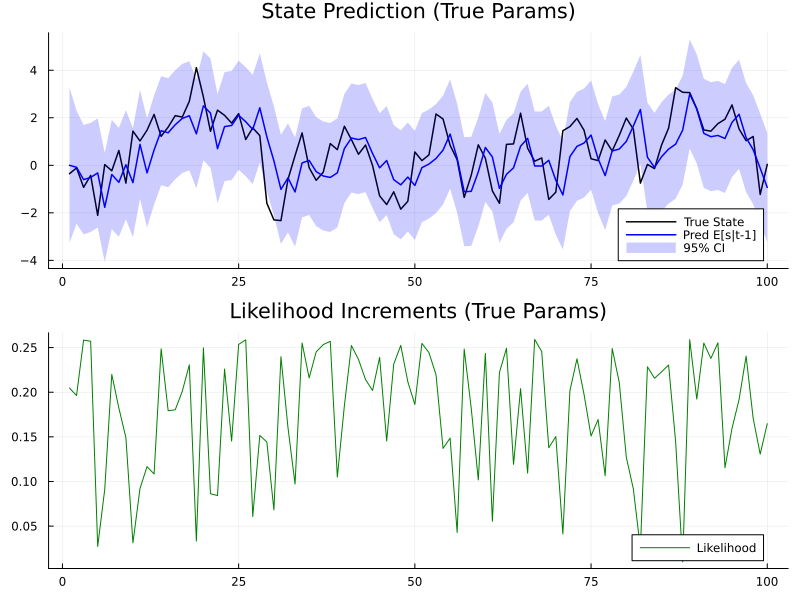
\includegraphics[width=\textwidth]{P2_e_true.png}
    \caption{(i) True Parameters: $\lambda=1$, $\phi=0.8$}
    \label{fig:kf_true}
  \end{minipage}
  \hfill
  \begin{minipage}
    {0.45\textwidth}
    \centering
    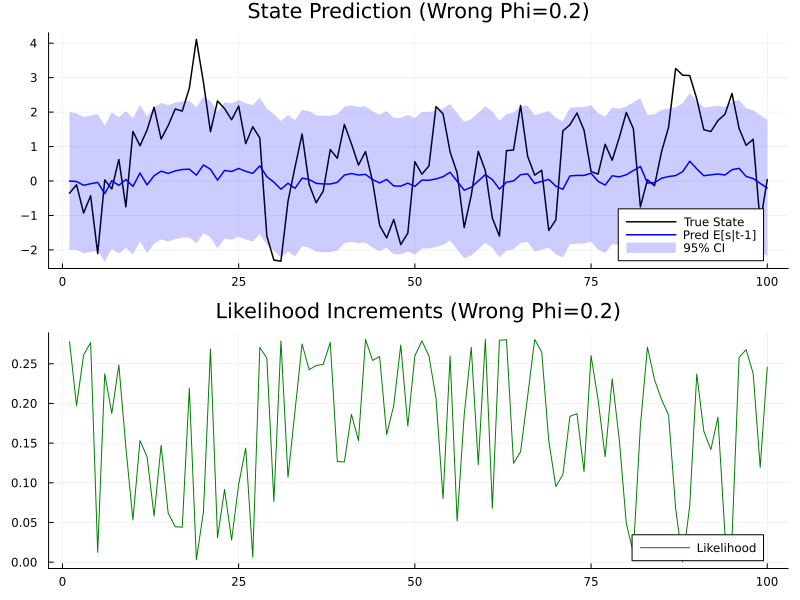
\includegraphics[width=\textwidth]{P2_e_wrong.png}
    \caption{(ii) Wrong Parameters: $\lambda=1$, $\phi=0.2$}
    \label{fig:kf_wrong}
  \end{minipage}
\end{figure}

The comparative analysis of the State-Space model simulations reveals the critical role of parameter consistency in filtering and inference.
In the first scenario, where the filter is initialized with the true data-generating parameters ($\lambda=1.0, \phi=0.8$),
the predicted state expectation $\mathbb{E}[s_t | Y_{1:t-1}]$ exhibits a high degree of correlation with the true state trajectory.
The filter successfully captures the persistence of the underlying process,
as the coefficient $\phi=0.8$ implies significant memory in the state transition equation $s_t = \phi s_{t-1} + \epsilon_t$.
Consequently, the one-step-ahead predictions effectively project current information into the future,
resulting in a tracking error that behaves as a stationary white noise process consistent with theoretical expectations.

Conversely, the second scenario employs a misspecified parameter ($\phi=0.2$),
leading to a severe degradation in filter performance.
Visually, the predicted state trajectory appears overly smoothed and rapidly mean-reverting,
failing to track the excursions of the true state away from zero.
This phenomenon occurs because the misspecified model assumes a near-white noise process with minimal persistence.
As a result, the filter attributes observed deviations largely to transient measurement noise $u_t$ rather than structural shocks $\epsilon_t$,
causing the predicted state to revert prematurely to the unconditional mean of zero.
This highlights the bias in state extraction introduced by underestimating the autoregressive parameter.

Furthermore, the discrepancy in the confidence intervals (shaded regions) illustrates the impact of misspecification on uncertainty quantification.
The width of the error bands is determined by the steady-state variance of the state, given by $\sigma^2_s = (1-\phi^2)^{-1}$.
The true model correctly estimates a larger unconditional variance ($\approx 2.78$),
producing wide confidence intervals that encompass the true realizations.
The misspecified model, however, implies a much lower variance ($\approx 1.04$),
resulting in "overconfident" narrow bands that are frequently violated by the true state.
This underestimation of risk leads to substantial drops in the likelihood function whenever the true state realizes a value outside these narrow bounds,
empirically demonstrating why Maximum Likelihood Estimation favors the parameter set that correctly balances prediction error against predicted uncertainty.

\subsection*{(f) \& (g) Grid Search for MLE of $\phi$}

\begin{lstlisting}[language=R]
  T_sizes = [50, 100, 500]
  phi_grid = range(0.01, 0.99, length=100)
  
  p_tmp = plot(xlabel="Phi", ylabel="Log-Likelihood",
              title="Log-likelihood vs Phi for different T",
              legend=:right, grid=true)
  
  colors = [:red, :blue, :green]
  for (i, T_val) in enumerate(T_sizes)
    _, y_T = simulate_ss(T_val, TRUE_LAM, TRUE_PHI)
    ll_vals = [kalman_filter(y_T, TRUE_LAM, p).total_ll for p in phi_grid]
    
    plot!(p_tmp, phi_grid, ll_vals,
          linewidth=2, color=colors[i],
          label="T=$T_val")
  end
  
  vline!(p_tmp, [TRUE_PHI], linewidth=1.5, linestyle=:dash, color=:black, label="True Phi")
  
  savefig(p_tmp, "P2_g_combined.png")
  display(p_tmp)
\end{lstlisting}

\begin{figure}[h!]
  \centering
  \includegraphics[width=0.85\textwidth]{P2_g_combined.png}
  \caption{Log-likelihood vs Phi for different T}
  \label{fig:ll_combined}
\end{figure}

\subsection*{(h) Numerical Optimization for MLE of $\phi$}
\begin{lstlisting}[language=R]
  using Optim, Printf

  open("P2_h.tex", "w") do f
      write(f, "\\begin{table}[htbp]\n")
      write(f, "\\centering\n")
      write(f, "\\caption{Comparison of Maximum Likelihood Estimates via Grid Search and Gradient-Based Optimization}\n")
      write(f, "\\label{tab:mle_comparison}\n")
      write(f, "\\begin{tabular}{cccc}\n")
      write(f, "\\toprule\n")
      write(f, "Sample Size & Grid Search MLE & Gradient Optimization MLE & Max Log-Likelihood \\\\\n")
      write(f, "\\midrule\n")
  
      for T_val in T_sizes
          Random.seed!(2025)
          _, y = simulate_ss(T_val, TRUE_LAM, TRUE_PHI)
  
          # ---------- 1) Grid Search ----------
          ll_vals = [kalman_filter(y, TRUE_LAM, p).total_ll for p in phi_grid]
          best_idx = argmax(ll_vals)
          grid_est = phi_grid[best_idx]
          grid_ll = ll_vals[best_idx]
  
          # ---------- 2) Gradient-based (LBFGS) ----------
          nll_vec(\theta::Vector) = -kalman_filter(y, TRUE_LAM, \theta[1]).total_ll
  
          function bounded_nll(\theta::Vector)
              if \theta[1] <= 0.0 || \theta[1] >= 1.0
                  return Inf
              end
              return nll_vec(\theta)
          end
  
          # Use grid estimate as initial guess
          initial_guess = [grid_est]
  
          # Use LBFGS optimization
          res = optimize(bounded_nll, initial_guess, LBFGS())
  
          optim_est = Optim.minimizer(res)[1]
          max_ll = -Optim.minimum(res)
  
          write(f, Printf.@sprintf("%d & %.3f & %.3f & %.1f \\\\\n",
              T_val, grid_est, optim_est, max_ll))
      end
  
      write(f, "\\bottomrule\n")
      write(f, "\\end{tabular}\n")
      write(f, "\\end{table}\n")
  end
\end{lstlisting}

\begin{table}[htbp]
\centering
\caption{Comparison of Maximum Likelihood Estimates via Grid Search and Gradient-Based Optimization}
\label{tab:mle_comparison}
\begin{tabular}{cccc}
\toprule
Sample Size & Grid Search MLE & Gradient Optimization MLE & Max Log-Likelihood \\
\midrule
50 & 0.792 & 0.796 & -92.3 \\
100 & 0.762 & 0.765 & -185.9 \\
500 & 0.782 & 0.784 & -911.6 \\
\bottomrule
\end{tabular}
\end{table}


The gradient-based optimization yields estimates that are virtually identical to those obtained via grid search.
The negligible differences between the two sets of estimates indicate that the log-likelihood surface is well-behaved and unimodal within the stationarity bounds,
allowing both methods to converge to the same local optimum.
This agreement validates the reliability of the gradient-based approach as an efficient alternative to grid search,
particularly beneficial in higher-dimensional parameter spaces where computational costs become prohibitive for exhaustive search methods.


\subsection*{(i) Correlated Errors: $\mathrm{Cov}(u_t,\varepsilon_t)=\rho$}

\paragraph{Autocovariance Function}
Let $u_t$ and $\varepsilon_t$ be jointly normal with $\mathrm{Cov}(u_t,\varepsilon_t)=\rho$. The autocovariance function of $y_t$ becomes:
\begin{align*}
  \gamma_y(0) & = \mathbb{V} [\lambda s_t + u_t] = \lambda^2 \mathbb{V} [s_t] +  \mathbb{V} [u_t] + 2\lambda\mathrm{Cov}(s_t,u_t) \\
              & = \frac{\lambda^2}{1-\phi^2} + 1 + 2\lambda\rho,                                                                  \\
  \gamma_y(1) & = \mathrm{Cov}(y_t,y_{t-1}) = \lambda^2\mathrm{Cov}(s_t,s_{t-1}) + \lambda\mathrm{Cov}(s_t,u_{t-1})               \\
              & = \frac{\lambda^2\phi}{1-\phi^2} + \lambda\phi\rho,                                                               \\
  \gamma_y(h) & = \lambda^2\mathrm{Cov}(s_t,s_{t-h}) = \frac{\lambda^2\phi^h}{1-\phi^2}, \quad h \geq 2.
\end{align*}

\paragraph{Identification}
The parameters are not fully identified. For $h \geq 2$, the ratio $\gamma_y(h)/\gamma_y(h-1) = \phi$ still identifies $\phi$.
Given $\phi$, we have two equations from $\gamma_y(0)$ and $\gamma_y(1)$:
\begin{align*}
  \gamma_y(0) & = \frac{\lambda^2}{1-\phi^2} + 1 + 2\lambda\rho,    \\
  \gamma_y(1) & = \frac{\lambda^2\phi}{1-\phi^2} + \lambda\phi\rho.
\end{align*}

These equations determine $\lambda^2$ and $\rho$, but $\lambda$ is identified only up to sign.
If $(\lambda,\rho)$ satisfies these equations, then $(-\lambda,-\rho)$ also satisfies them.
Thus, the parameter sets $(\lambda,\phi,\rho)$ and $(-\lambda,\phi,-\rho)$ are observationally equivalent.

\paragraph{ARMA(1,1) Representation}
Applying $(1-\phi L)$ to $y_t$:
\[
  (1-\phi L)y_t = \lambda(1-\phi L)s_t + (1-\phi L)u_t = \lambda\varepsilon_t + u_t - \phi u_{t-1}.
\]
Let $w_t = \lambda\varepsilon_t + u_t - \phi u_{t-1}$. Then $y_t = \phi y_{t-1} + w_t$, where $w_t$ has autocovariances:
\begin{align*}
  \gamma_w(0) & =  \mathbb{V} [\lambda\varepsilon_t + u_t - \phi u_{t-1}] = \lambda^2 + 1 + \phi^2 + 2\lambda\rho, \\
  \gamma_w(1) & = \mathrm{Cov}(w_t,w_{t-1}) = -\phi(1+\lambda\rho),                                                \\
  \gamma_w(h) & = 0, \quad h \geq 2.
\end{align*}
Thus $w_t$ is MA(1): $w_t = \nu_t + \theta\nu_{t-1}$ with $\nu_t \sim \mathrm{WN}(0,\sigma_\nu^2)$, where $\theta$ and $\sigma_\nu^2$ satisfy:
\[
  \sigma_\nu^2(1+\theta^2) = \lambda^2 + 1 + \phi^2 + 2\lambda\rho, \quad
  \sigma_\nu^2\theta = -\phi(1+\lambda\rho).
\]
Solving these yields the ARMA(1,1) representation $y_t = \phi y_{t-1} + \nu_t + \theta\nu_{t-1}$.


\subsection*{(j) Generalized Kalman Filter with Correlation}

Let $\mathrm{Cov}(\varepsilon_t,u_t) = \rho$. Given information up to $t-1$, denote:
\[
  m_{t-1|t-1} = \mathbb{E}[s_{t-1} \mid Y_{1:t-1}], \quad
  P_{t-1|t-1} = \mathbb{V}[s_{t-1} \mid Y_{1:t-1}].
\]

\paragraph{Prediction Step:}
\[
  m_{t|t-1} = \phi\,m_{t-1|t-1}, \quad
  P_{t|t-1} = \phi^2 P_{t-1|t-1} + 1.
\]

\paragraph{Innovation:}
The forecast error for $y_t$ is:
\[
  v_t = y_t - \lambda m_{t|t-1}.
\]
Its conditional variance is:
\begin{align*}
  F_t & = \mathbb{V}[v_t \mid Y_{1:t-1}]                                                         \\
      & = \mathbb{V}[\lambda(s_t - m_{t|t-1}) + u_t \mid Y_{1:t-1}]                              \\
      & = \lambda^2 P_{t|t-1} + 1 + 2\lambda\,\mathrm{Cov}(s_t - m_{t|t-1}, u_t \mid Y_{1:t-1}).
\end{align*}
Since $s_t - m_{t|t-1} = \phi(s_{t-1} - m_{t-1|t-1}) + \varepsilon_t$ and $s_{t-1} - m_{t-1|t-1}$ is uncorrelated with $u_t$, we have:
\[
  \mathrm{Cov}(s_t - m_{t|t-1}, u_t \mid Y_{1:t-1}) = \mathrm{Cov}(\varepsilon_t, u_t) = \rho.
\]
Thus,
\[
  F_t = \lambda^2 P_{t|t-1} + 1 + 2\lambda\rho.
\]

\paragraph{Kalman Gain:}
The covariance between the state and the innovation is:
\begin{align*}
  \mathrm{Cov}(s_t, v_t \mid Y_{1:t-1})
   & = \mathrm{Cov}(s_t, \lambda(s_t - m_{t|t-1}) + u_t \mid Y_{1:t-1})                \\
   & = \lambda\,\mathbb{V}[s_t \mid Y_{1:t-1}] + \mathrm{Cov}(s_t, u_t \mid Y_{1:t-1}) \\
   & = \lambda P_{t|t-1} + \rho.
\end{align*}
The Kalman gain is then:
\[
  K_t = \frac{\mathrm{Cov}(s_t, v_t \mid Y_{1:t-1})}{F_t} = \frac{\lambda P_{t|t-1} + \rho}{F_t}.
\]

\paragraph{Update Step:}
\begin{align*}
  m_{t|t} & = m_{t|t-1} + K_t v_t,                                   \\
  P_{t|t} & = P_{t|t-1} - K_t\,\mathrm{Cov}(s_t, v_t \mid Y_{1:t-1}) \\
          & = P_{t|t-1} - K_t(\lambda P_{t|t-1} + \rho).
\end{align*}

\paragraph{Log-Likelihood Increment:}
\[
  \log p(y_t \mid Y_{1:t-1}) = -\frac{1}{2}\left(\log(2\pi) + \log F_t + \frac{v_t^2}{F_t}\right).
\]

\end{document}